\documentclass[12pt]{article}
% basic preamble for any kind of document

\usepackage{xcolor}
\usepackage{amsmath}
\usepackage{geometry}
\usepackage{graphicx}
\usepackage{appendix}
\usepackage{setspace} % double spacing
					  % use \doublespacing

\setlength{\parindent}{0pt}

\definecolor{blue}{RGB}{0,114,178}
\newcommand{\fix}[1]{\textcolor{blue}{\textbf{#1}}}

\usepackage{titlesec} % what does this do?

\usepackage{tabularx}
\usepackage{subfig}
\usepackage{ragged2e}
\usepackage{amstext}

\author{Emily Case}
\date{\today}
\title{Applied Metrics PS2: Matching and Weighting}

% -------------------------------------------------------------- % 
\begin{document}
\maketitle

\textbf{Question 1.} Regressing 1978 real earnings on the (original) treated variable yields an estimate that those who received the experiment treatment earn \$818.70 more than those who weren't treated, controlling for other demographic information. The experimental effect might be different for different kinds of people, so we want to include covariates to improve the estimated experimental impact. \\
\begin{table}[htbp]\centering
\caption{Question 1\label{q1}}
\begin{tabular}{l*{1}{c}}
\toprule
            &\multicolumn{1}{c}{1978 real earnings}\\
\midrule
treated     &      818.70\\
            &    (487.83)\\
\addlinespace
age         &     -145.92\\
            &    (200.76)\\
\addlinespace
age2        &        2.80\\
            &      (3.25)\\
\addlinespace
educ        &      206.81\\
            &    (165.45)\\
\addlinespace
black       &    -1461.26\\
            &    (734.32)\\
\addlinespace
hisp        &      100.48\\
            &    (958.57)\\
\addlinespace
married     &      133.91\\
            &    (660.02)\\
\addlinespace
nodegree    &     -405.91\\
            &    (752.08)\\
\addlinespace
re74        &        0.09\\
            &      (0.11)\\
\addlinespace
re75        &        0.08\\
            &      (0.12)\\
\addlinespace
\_cons      &     5648.81\\
            &   (3757.50)\\
\midrule
\(N\)       &         722\\
\bottomrule
\multicolumn{2}{l}{\footnotesize Standard errors in parentheses}\\
\end{tabular}
\end{table}


\bigskip 
\textbf{Question 2. Drop the experimental treatment group.}

\bigskip
\textbf{Question 3.}
I define \texttt{treated2} as 0 when an observation is in the CPS group, and 1 when an observation is in the experiment's control group. Running probits with \texttt{treated2} as the dependent variable on both the coarse and rich set of independent variables yields the results in Table \ref{q3}. 
\begin{table}[htbp]\centering
\caption{Probit models\label{q3}}
\begin{tabular}{l*{2}{c}}
\toprule
            &\multicolumn{1}{c}{Coarse}&\multicolumn{1}{c}{Rich}\\
\midrule
treated2    &            &            \\
age         &      0.2532&      0.3225\\
            &      (0.03)&      (0.03)\\
\addlinespace
age2        &     -0.0045&     -0.0055\\
            &      (0.00)&      (0.00)\\
\addlinespace
educ        &      0.0169&      0.0178\\
            &      (0.02)&      (0.02)\\
\addlinespace
black       &      1.9899&      1.9504\\
            &      (0.08)&      (0.08)\\
\addlinespace
hisp        &      0.9733&      0.9775\\
            &      (0.10)&      (0.11)\\
\addlinespace
married     &     -1.1011&     -0.9091\\
            &      (0.08)&      (0.09)\\
\addlinespace
nodegree    &      1.1327&      1.0712\\
            &      (0.10)&      (0.10)\\
\addlinespace
re74        &            &     -0.0000\\
            &            &      (0.00)\\
\addlinespace
re75        &            &     -0.0001\\
            &            &      (0.00)\\
\addlinespace
\_cons      &     -6.3580&     -7.1081\\
            &      (0.48)&      (0.51)\\
\midrule
\(N\)       &       16417&       16417\\
\bottomrule
\multicolumn{3}{l}{\footnotesize Standard errors in parentheses}\\
\end{tabular}
\end{table}

\\\\
Some combinations of covariates perfectly determine if someone is in the experimental group or not. None of the observations in the experimental sample are completely determined. There are 727 observations that are \textit{not} in the experimental sample (i.e. they are in the CPS sample) that are completely determined using the coarse variables, and 1359 using the rich set of variables. This is important because the observations that are completely determined, we know there is no probability that they would be part of the \textit{other} group, which would be important for propensity score matching. They are not helpful to us when we match. 


\newpage
\textbf{Question 4.} 
% What do the descriptive statistics suggest about the common support condition in these data?
The descriptive statistics of the estimated propensity scores by group suggest that we do not anticipate having an issue with the common support for the coarse scores. We might need to impose the common support condition for the rich scores, since they have different maxima across groups. 
\begin{table}[h!]
\caption{Looking at the common supports}
	\label{q4}
\begin{center}
\begin{tabular}{lrccc}
\toprule
& & Minimum & Mean & Maximum \\
\addlinespace
\hline
\multicolumn{2}{l}{\textit{coarse scores}} & & & \\
& CPS group & 0 & .01641 & .6872 \\
& control group & .00008 & .3873 & .6872 \\ \addlinespace
\multicolumn{2}{l}{\textit{rich scores}} & & & \\
& CPS group & 0 & .01545 & .7886000000000001 \\
& control group & 0 & .42483 & .8024 \\
\bottomrule
\end{tabular}
\end{center}
\end{table}


% What do they suggest about the comparability of the CPS comparison group?
The CPS comparison group is pretty different from the control group. Despite covering more or less the same support, notice that the mean propensity scores for the experimental control group and the CPS group are very different. The CPS group propensity scores are much more highly concentrated around 0. 


\bigskip

\textbf{Question 5.}
% What do the histograms suggest about the common support condition in these data?
The histograms in Figures \ref{q5a} (on page \pageref{q5a}) and \ref{q5b} (on page \pageref{q5b}) suggest that there is not a big common support issue, but that there are underlying differences in the control group sample and the CPS sample, similarly to question 4. 
% What do they suggest about the comparability of the CPS comparison group?
\\\\
Visually, it looks like the histogram for the rich scores, Figure \ref{q5b}, has slightly more similarities between the experimental control group and the CPS group. 
\begin{figure}
	\centering
	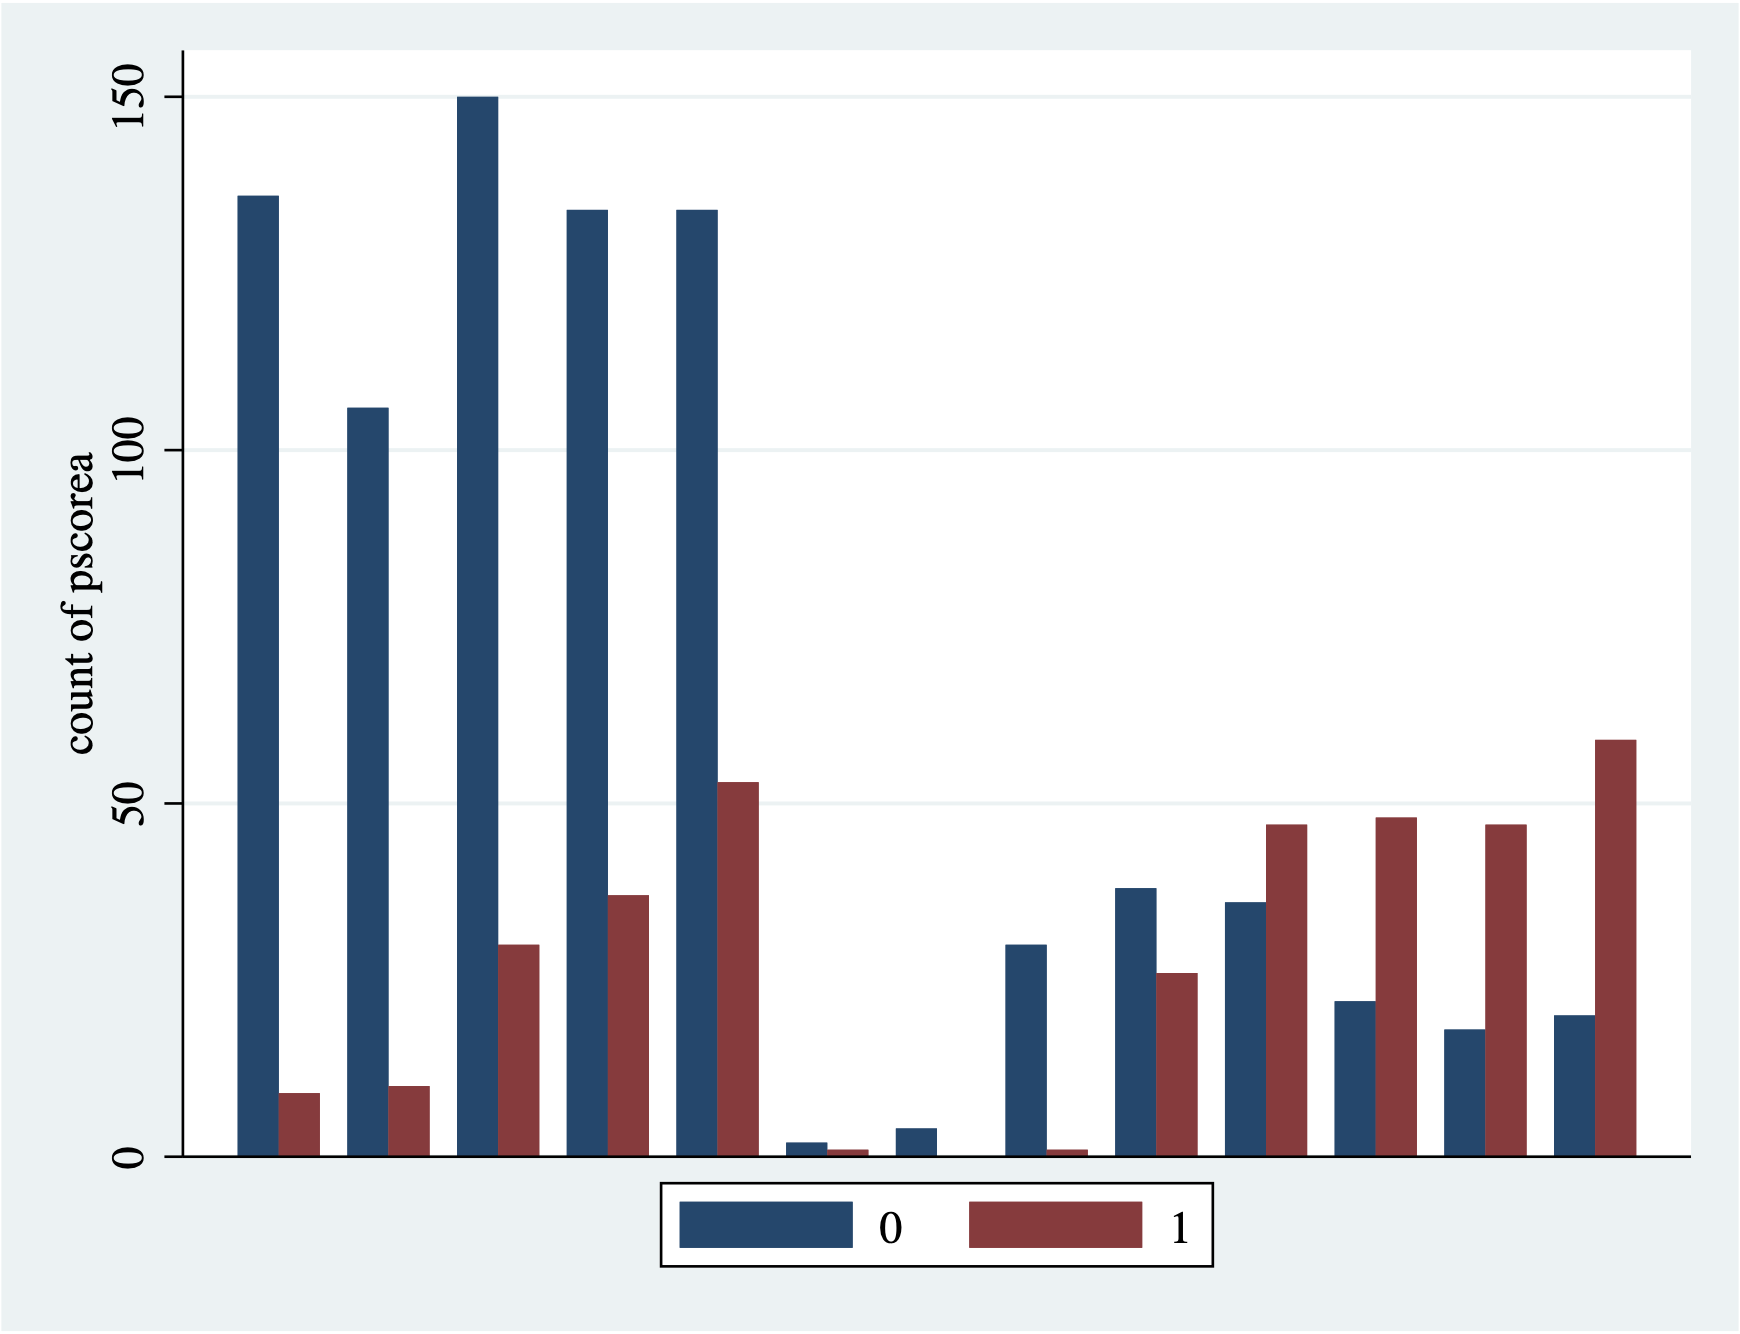
\includegraphics[scale = 0.2]{q4_pscorea}
	\caption{Counting observations of control group and CPS group in propensity score bins, using the coarse propensity scores. I omit observations in the first bin, in order to make the other bins visible. }
	\label{q5a}
\end{figure}
\begin{figure}
	\centering
	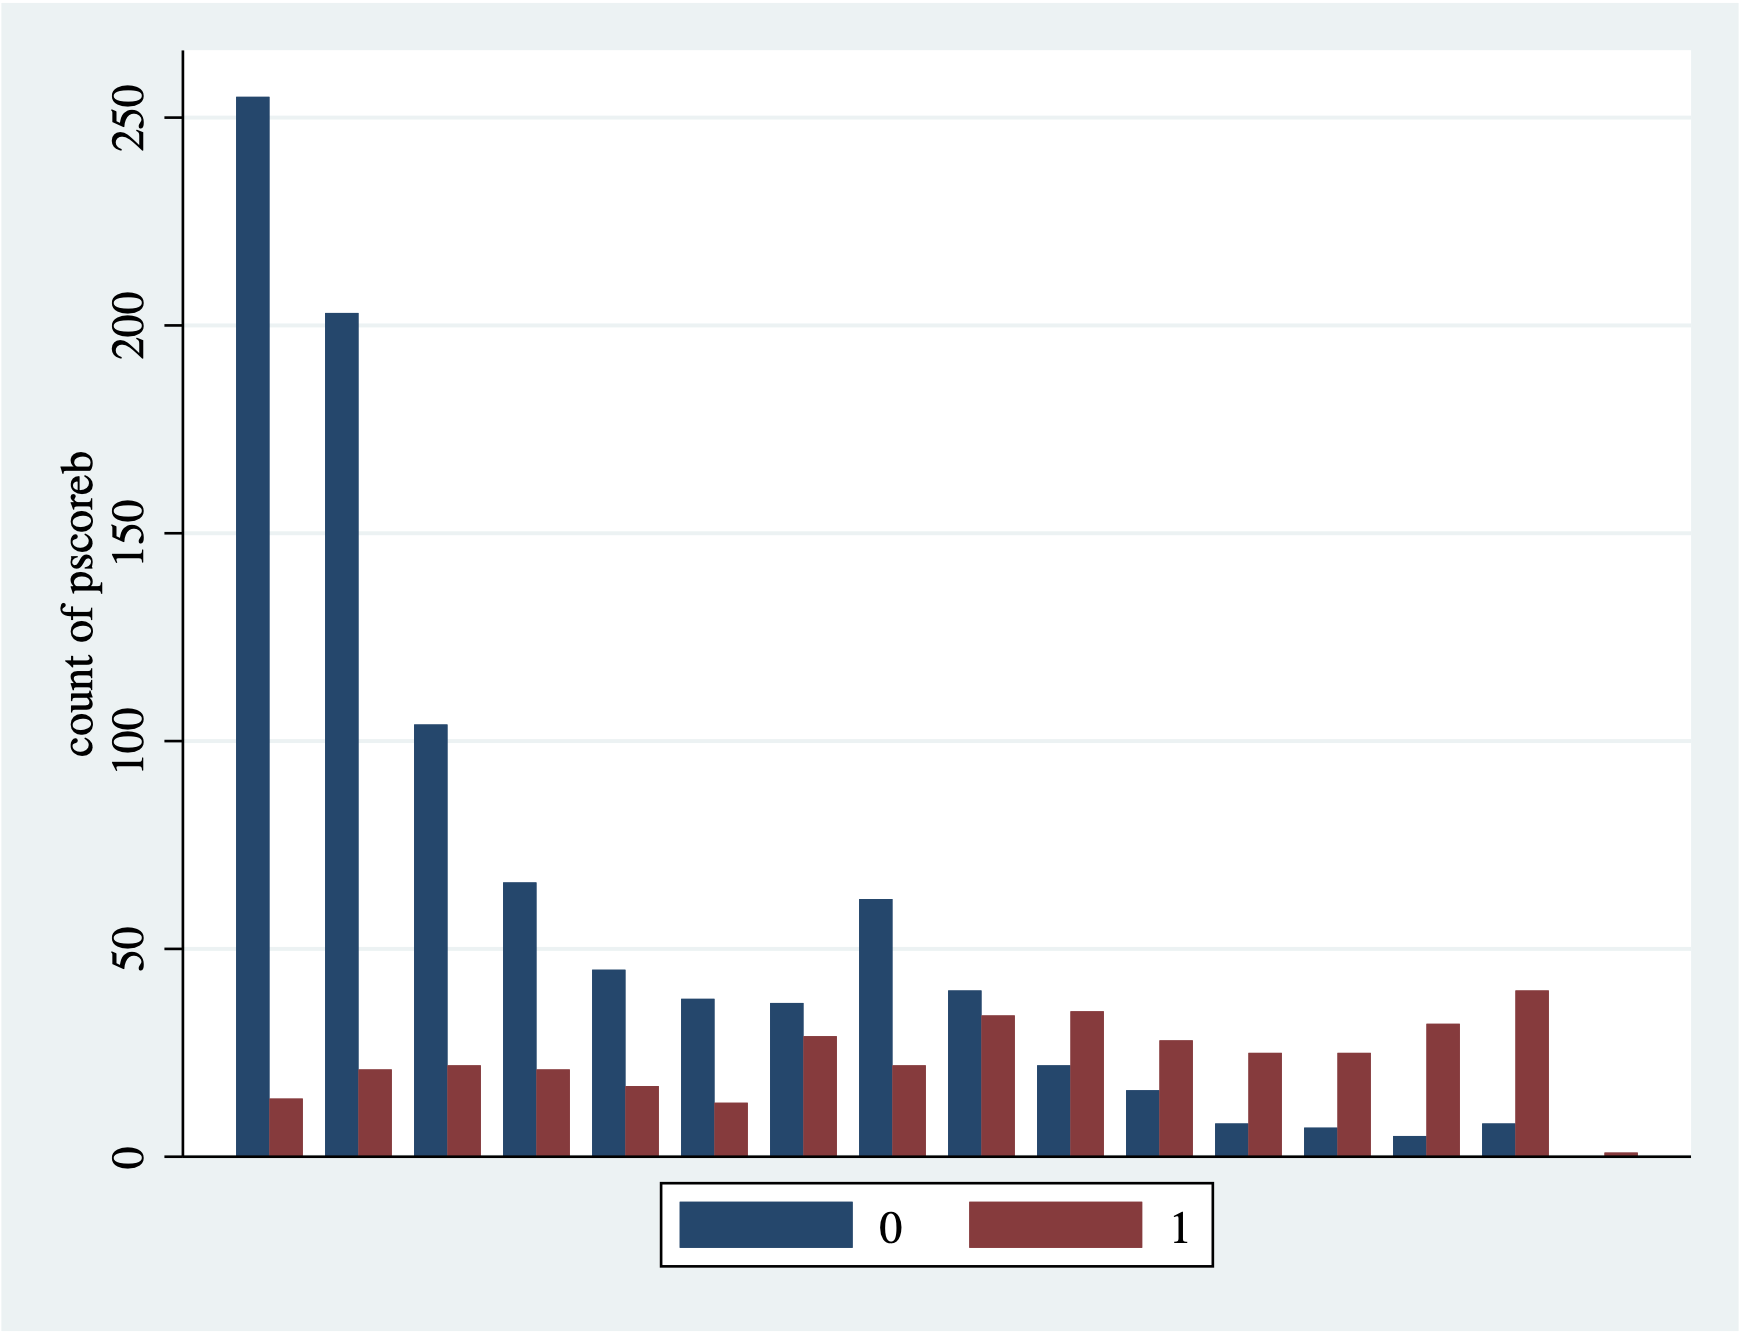
\includegraphics[scale = 0.2]{q4_pscoreb.png}
	\caption{Counting observations of control group and CPS group in propensity score bins, using the rich propensity scores. I omit observations in the first bin, in order to make the other bins visible. }
	\label{q5b}
\end{figure}

\newpage
\textbf{Question 6. Impose common support condition, no replacement.}\\
% Which observations are dropped?
No observations were dropped using the coarse scores, and 7 were dropped using the rich scores. The observations off the support (for rich scores) have propensity scores that are above 0.7886, which is the minimum of 0.7886 and 0.8024 (the two maxima propensity scores). 
\\\\
% How close are the resulting estimates to the experimental impact estimate?
The experimental impact from Table \ref{q1} was \$818.70. The results for coarse and rich scores are below, in Table \ref{q6}.  Using coarse scores, the experimental group is estimated to have \$4,439 less real earnings in 1978 compared to the CPS group. Using rich scores, they are estimated to have \$2,340 less than the CPS group. We want the differences to be close to zero... both these scores are clearly very far away from zero. 
\\\\
% Do the rich scores that contain pre-treatment earnings perform better (i.e., result in lower bias estimates) than the coarse scores that do not?
The rich scores do better by about \$2,000, but again, still pretty far away from zero. 
\begin{table}[h!]
\caption{Using \texttt{psmatch2} (questions 6 and 7)}
	\label{q6}
\begin{center}
\begin{tabular}{lrlllll}
\toprule
&& \multicolumn{2}{c}{\textbf{No replacement}} && \multicolumn{2}{c}{\textbf{Replacement}}\\ 
& & Difference & S.E. && Difference & S.E. \\
\addlinespace
\hline
\addlinespace
\multicolumn{2}{l}{\textit{coarse scores}} && & &&\\
& Unmatched & -9756.6 & 470.2 && -9756.6 & 470.2\\
& ATT & -4439.1 & 486.5 && -3677 & 934.5 \\ \addlinespace
\multicolumn{2}{l}{\textit{rich scores}} && & &&\\
& Unmatched & -9756.6 & 470.2 && -9756.6 & 470.2\\
& ATT & -2340.8 & 449.4 && -1516 & 707.6 \\
\bottomrule
\end{tabular}
\end{center}
\end{table}


\bigskip
\textbf{Question 7. Repeat question 6 but with replacement. }\\
When we allow for nearest neighbors to be reused for matching, the estimated differences for coarse and rich scores (in Column 2 of Table \ref{q6}) decrease compared to when we did not allow for replacement. They are still pretty far off from zero, but we are closer to zero as a result of more flexibility allowing better matches. 
\\\\
This makes sense when you think about the high concentration of CPS observations with propensity scores close to zero. Without replacement, when we want to match the control group scores with \textit{high} propensity scores, we run out of CPS observations with high propensity scores, and have to make worse matches. When we allow replacement, it gets a little bit better. 

\bigskip
\textbf{Question 8.}
\begin{table}[h!]
\caption{Standardized differences (question 8)}
	\label{q8}
\begin{center}
\begin{tabular}{rccc}
\toprule
& Raw data & Single NN with replacement & Reduced bias by \\
\addlinespace
\hline
\addlinespace
\texttt{re74} & 126.32 & -9.1 & 92.83\% \\ \addlinespace
\texttt{re75} & 141.35 & -7.34 & 94.8\% \\
\bottomrule
\end{tabular}
\end{center}
\end{table}

% Estimate the standardized difference in “real earnings in 1974” and “real earnings in 1975” based on the raw data 
% and based on the rich scores and single nearest neighbour matching with replacement. 
The standardized differences for raw data and for the rich scores using single nearest neighbor matching with replacement are in Table \ref{q8} on page \pageref{q8}. 
% What is the proportionate reduction in the standardized “bias” from the conditioning? 
When we match using the rich scores, the bias is reduced significantly (see the third column).

\bigskip
\textbf{Question 9 and 10.}
% Describe the resulting impact estimates. 
Results for the Gaussian kernel and local linear matching are in Table \ref{q10} on page \pageref{q10}. Compared to question 6 and 7, using a Gaussian kernel generally worsens the difference estimates, while using local linear matching improves them.\\\\ 
% How do the estimates change as the bandwidth increases? 
In Gaussian kernels, the bandwidth of 0.02 is the best in the sense that it is close to zero, but we also do notice the trade off of a higher standard error as a result. As bandwidth increases, the difference estimates get larger in magnitude. Here we want a smaller bandwidth. 
\\\\
Using local linear matching, in absolute value the bandwidth of 2.0 is closest to zero, and performs better than any of the difference estimates so far. 
% How do the estimates differ from the single nearest neighbor matching with replacement estimates obtained in Problem 7?
\begin{table}[h!]
\caption{Problem 10}
	\label{q10}
\begin{center}
\begin{tabular}{ll}
\toprule
Cutoff value & Correct prediction rate \\
\toprule
0.5 & 0 \\
loan take up fraction  & 0 \\
\bottomrule
\end{tabular}
\end{center}
\end{table}


\newpage
\textbf{Question 11 and 12.}
Results for 11 and 12 are in Table \ref{q12} on page \pageref{q12}. Running a linear regression of real earnings in 1978 using all of the observations in the control group and the CPS comparison group in column 1 shows an estimated bias of -\$1,853.39, which is higher than our closest efforts from matching. 
\\\\
If instead we use only the untreated (CPS) observations, I get a very similar estimated bias of -\$1851.55. % I am not sure why them being similar matters.

\begin{table}[htbp]\centering
\def\sym#1{\ifmmode^{#1}\else\(^{#1}\)\fi}
\caption{Problem 12: probit models \label{q12}}
\begin{tabular}{l*{2}{c}}
\toprule
     &\multicolumn{1}{c}{(1)}&\multicolumn{1}{c}{(2)}\\
     &\multicolumn{1}{c}{no interaction}&\multicolumn{1}{c}{interaction}\\
\midrule
Client took a loan&                     &                     \\
Client age&      0.0002         &      0.0009         \\
     &    (0.0086)         &    (0.0087)         \\
\addlinespace
Client marital status=1&      0.0495         &      0.1557         \\
     &    (0.2141)         &    (0.2807)         \\
\addlinespace
Client education&     -0.0146         &     -0.0154         \\
     &    (0.0166)         &    (0.0167)         \\
\addlinespace
Household size&     -0.0476         &     -0.0502         \\
     &    (0.0379)         &    (0.0381)         \\
\addlinespace
Household income&      0.0000         &      0.0000         \\
     &    (0.0000)         &    (0.0000)         \\
\addlinespace
Client is Muslim=1&     -0.0326         &      0.2059         \\
     &    (0.1468)         &    (0.4206)         \\
\addlinespace
Client is Hindi&     -0.1100         &     -0.1143         \\
     &    (0.2152)         &    (0.2153)         \\
\addlinespace
Treated&      0.1751         &      0.1820         \\
     &    (0.1419)         &    (0.1424)         \\
\addlinespace
Client marital status=1 $\times$ Client is Muslim=1&                     &     -0.2709         \\
     &                     &    (0.4481)         \\
\addlinespace
Constant&     -0.8527         &     -0.9589         \\
     &    (0.4592)         &    (0.4939)         \\
\midrule
Observations&         532         &         532         \\
\bottomrule
\multicolumn{3}{l}{\footnotesize Standard errors in parentheses}\\
\multicolumn{3}{l}{\footnotesize \sym{*} \(p<0.05\), \sym{**} \(p<0.01\), \sym{***} \(p<0.001\)}\\
\end{tabular}
\end{table}

	% bias estimate is the treated2 coeff in col(1) for q11 
	% for 12: we are only calculating for treated2= 1, and the coeff are changing so that tells us that there's something else happening
	
\bigskip
\textbf{Question 13.} Using the formulas for the ATT using inverse probability weighting on page 19 of the notes, I get an average treatment effect on the treated of -\$1420.38 for unscaled weights and -\$1996.47 using scaled weights. Normalizing the weights to sum to one in the sample is the ``preferred'' version.  

\end{document}
